\begin{figure}[t!]
	\centering    
	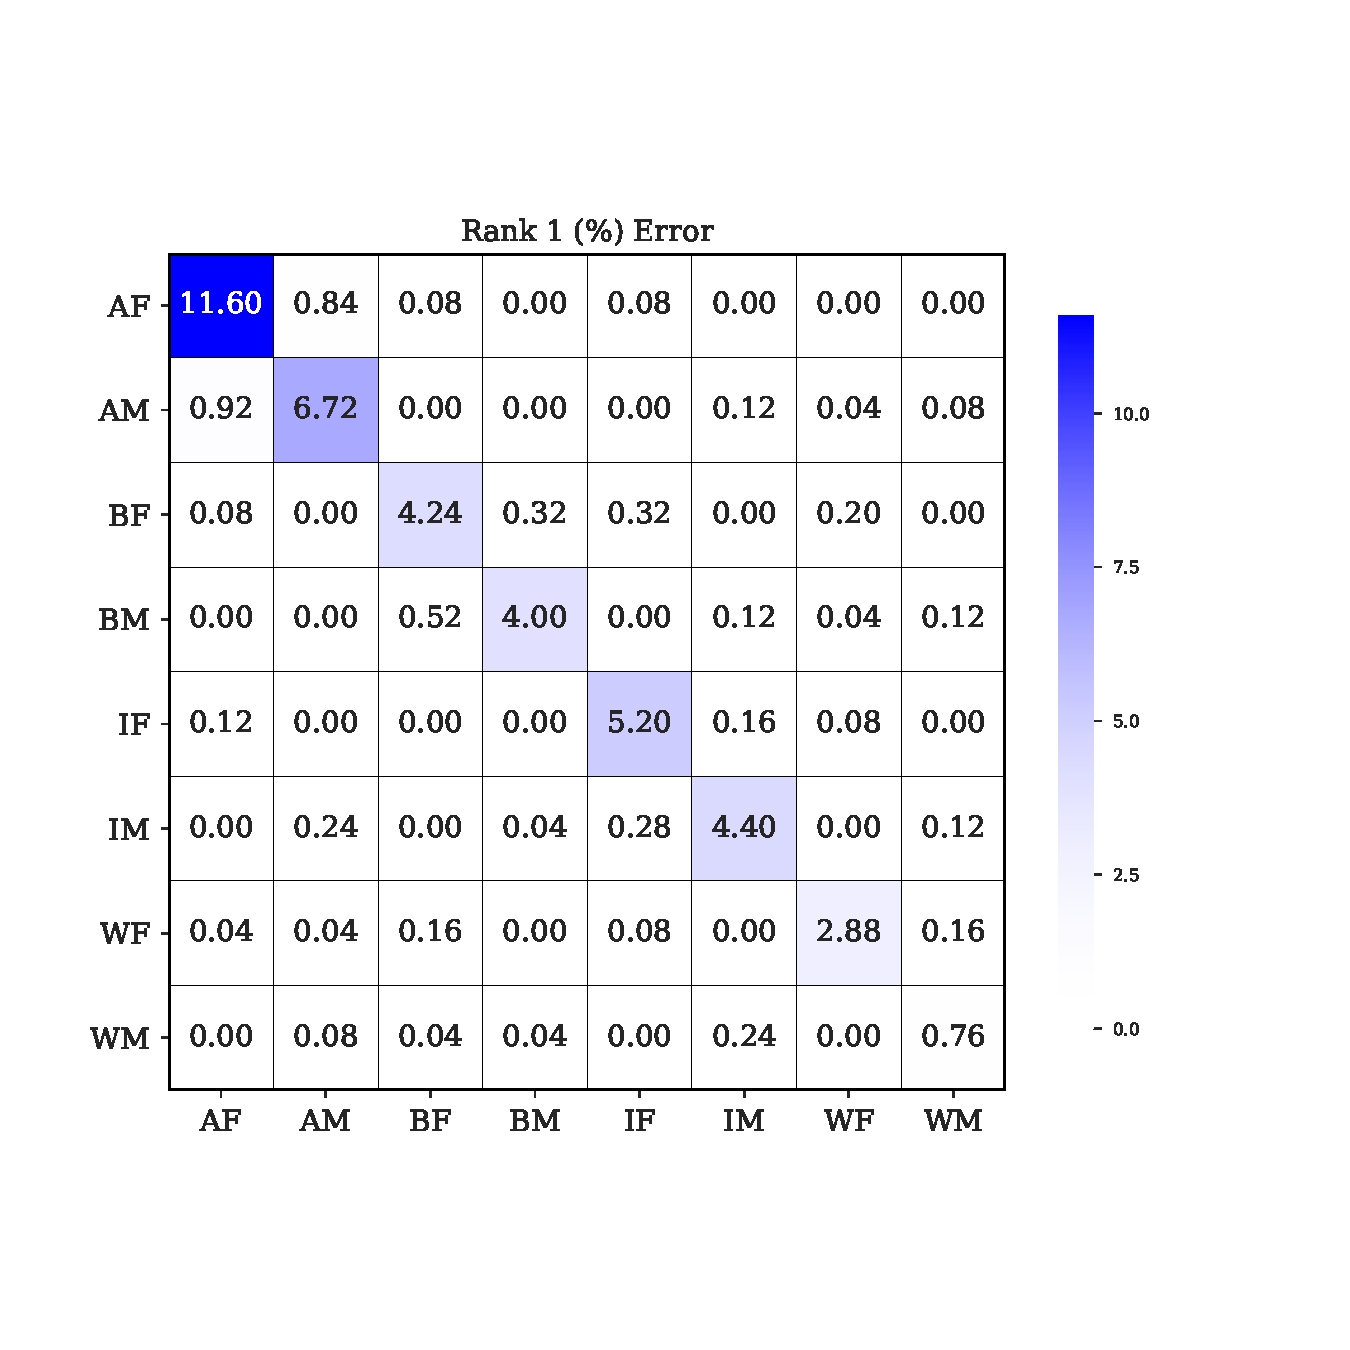
\includegraphics[width=\linewidth]{images/confusion.pdf}
		\caption{\small{\textbf{Confusion matrix.} Percent error (Rank 1) for all faces of \gls{bfw} queried against all others. Notice errors concentrate within a subgroup, consistent with the \gls{sdm} in Fig.~\ref{fig:detection-model} (\ie \gls{af} show worst performance, and is mostly confused with faces of the same demographic). This plot is evidence that while race/ethnicity may be challenging to define, the subgroups are meaningful.}}
		\label{fig:confusion} 
		\vspace{-5mm}
\end{figure} 

\section{Results and Analysis}
An {\em off-the-shelf} \gls{cnn} was used throughout to control the model across all experiments. For this, Sphereface~\cite{liu2017sphereface} trained on CASIA-Web~\cite{yi2014learning}, and evaluated on \gls{lfw}~\cite{LFWTech} (\%99.22 accuracy), encoded all of the faces.\footnote{\href{$https://github.com/clcarwin/sphereface\_pytorch$}{https:\/\/github.com\/clcarwin\/sphereface\_pytorch}} Following~\cite{liu2017sphereface}, upon applying an affine transformation to align faces according to pre-defined eye locations, each face got fed through the network twice, the original and horizontally flipped. The two features were fused by concatenation.

Additional \gls{cnn}-based models demonstrate the same phenomena: proportional to the overall model performance, exact in which the ordering subgroups in sensitivity in scores space (Appendix~\ref{app:sec:other:models}).
% Specifically, we analyze three \glspl{cnn} variants: we encode faces using VGG-16~\cite{simonyan2014very},  50-layer residual network (\ie ResNet-50)~\cite{he2016deep}, and \gls{senet} (\ie SENet-50)~\cite{hu2018squeeze}, with results of only the latter (\ie the best performing \gls{senet}) model used throughout the main paper. Results for the other two, alongside \gls{senet} for comparison, are in the Supplemental Material.


\glsunset{am}\glsunset{af}\glsunset{bm}\glsunset{bf}\glsunset{im}\glsunset{if}\glsunset{wm}\glsunset{wf}




% \vspace{-2pt}
\subsection{Score Analysis}
Fig.~\ref{fig:detection-model} shows score distributions for faces of the same identity (\ie \emph{Genuine}) and different (\ie \emph{Imposter}), with \gls{sdm}s split by subgroup. Observe that scores of imposters  approximately distribute about a peak of zero independent of subgroup, with slightly different standard deviation. Observe that the broadness in score distribution of the \emph{genuine} pairs varies across subgroups. Asian Fem
Fig.~\ref{fig:confusion} shows the confusion matrix of the subgroups. A vast majority of errors occurs in intra-subgroup. It is interesting to note that while the definition of  each group  based on ethnicity and race may not be crisply defined, the confusion matrix indicates that in practice the \gls{cnn} finds that the groups are effectively separate. The categories are, therefore, meaningful in the context of \gls{fr}.


\subsection{\gls{det} analysis}
\glsunset{m}
\glsunset{f}

\gls{det} curves averaged across 5-folds show per-subgroup trade-offs (Fig.~\ref{fig:detcurves}). Note that \gls{m} perform better than \gls{f}, precisely as one would expect from the tails of score-distributions for \emph{genuine} pairs (Fig.~\ref{fig:detection-model}). \Gls{af} and \gls{if} perform the worst.


 
\begin{table}[t!]
\glsunset{tar}
\glsunset{far}
\caption{\small{\textbf{\gls{tar} at intervals of \gls{far}}. For each subgroup, and overall average \gls{far}, listed are the \gls{tar} scores for a global threshold (top) and the proposed category-based threshold (bottom). Higher is better. The proposed shows improvement in all cases.}}\label{tab:ethnicy-far} 
 \vspace{-2mm}
\begin{center}
\begin{tabular}{l c c c c c}
     \gls{far} & 0.3 & 0.1 & 0.01 & 0.001 & 0.0001\\\midrule
    \multirow{2}{.1mm}{\textbf{\gls{af}}} &0.990 & 0.867 & 0.516 & 0.470 & 0.465\\[-4pt]
        &1.000 & 0.882 & 0.524 & 0.478 & 0.474\\[-1pt]
    \multirow{2}{3mm}{\textbf{\gls{am}}} &0.994 & 0.883 & 0.529 & 0.482 & 0.477\\[-4pt]
        &1.000 & 0.890 & 0.533 & 0.486 & 0.482\\[-1pt]
    \multirow{2}{3mm}{\textbf{\gls{bf}}} &0.991 & 0.870 & 0.524 & 0.479 & 0.473\\[-4pt]
        &1.000 & 0.879 & 0.530 & 0.484 & 0.480\\[-1pt]
    \multirow{2}{3mm}{\textbf{\gls{bm}}} &0.992 & 0.881 & 0.526 & 0.480 & 0.474\\[-4pt]
        &1.000 & 0.891 & 0.532 & 0.485 & 0.480\\[-1pt]
    \multirow{2}{3mm}{\textbf{\gls{if}}} &0.996 & 0.881 & 0.532 & 0.486 & 0.481\\[-4pt]
        &1.000 & 0.884 & 0.534 & 0.488 & 0.484\\[-1pt]
    \multirow{2}{3mm}{\textbf{\gls{im}}} &0.997 & 0.895 & 0.533 & 0.485 & 0.479\\[-4pt]
        &1.000 & 0.898 & 0.535 & 0.486 & 0.481\\[-1pt]
    \multirow{2}{3mm}{\textbf{\gls{wf}}} &0.988 & 0.878 & 0.517 & 0.469 & 0.464\\[-4pt]
        &1.000 & 0.894 & 0.526 & 0.478 & 0.474\\[-1pt]
    \multirow{2}{3mm}{\textbf{\gls{wm}}} &0.989 & 0.896 & 0.527 & 0.476 & 0.470\\[-4pt]
        &1.000 & 0.910 & 0.535 & 0.483 & 0.478\\[-1pt]
    \midrule
    \multirow{2}{3mm}{\textbf{Avg.}} &0.992 & 0.881 & 0.526 & 0.478 & 0.474\\[-4pt]
        &1.000 & 0.891 & 0.531 & 0.483 & 0.479\\[-10pt]
\end{tabular}
\end{center}
\glsreset{tar}
\glsreset{far}
 \vspace{-3mm}

\end{table}


The gender-based \gls{det} curve shows a difference in performances between \gls{m} and \gls{f} with a fixed threshold (dashed-line). Similar effects exist for the other curves as well (lines omitted to declutter). For many \gls{fr} applications, systems are operated at the highest \gls{fpr} allowed, so the line of constant threshold indicates that a single threshold produces different operating points (\ie \gls{fpr}), which is undesirable.  The difference in \gls{fpr} is approximately a factor of two-- quite large indeed. If this is the case in an industrial system, one would expect a difference in about double the false positives to be reported on based on subgroup alone. The potential ramifications of such a bias should not be overlooked, which it has not as of lately-- gaining interest of even main-stream media ~\cite{england2019,snow2018}.


\subsection{Verification threshold} \label{subsec:analysis:verification}
We seek to reduce the bias between subgroups. Such that an operating point (\ie \gls{fpr}) is constant across subgroups. To accomplish that, we used a per subgroup threshold. In \gls{fv}, we consider one image as the query and all others as test. For this, the ethnicity of the query image is assumed. We can then examine the \gls{det} curves and pick the best threshold per subgroup for a certain \gls{fpr}.

We evaluated \gls{tar} for specific \gls{far} values. As described in Section~\ref{subsec:pf}, the verification experiments were 5-fold, with no overlap in subject ID between folds. Results reported are averaged across folds in all cases and are shown in Table~\ref{tab:ethnicy-far}. For each subgroup, the \gls{tar} of using a global-threshold is reported (upper row), as well as using the optimal per subgroup threshold (lower row). 

Even for lower \gls{far}, there are notable improvements, often of the order of 1\%, which can be challenging to achieve when \gls{far} is near $\geq$90\%. More importantly, each subgroup has the desired \gls{fpr}, so that substantial differences in \gls{fpr} will remain unfounded. We further experimented using ethnicity estimators and using the ethnicity of both query and test image, which yielded similar results to those reported here (results not shown).

\begin{figure}[t!] 
	\centering    
	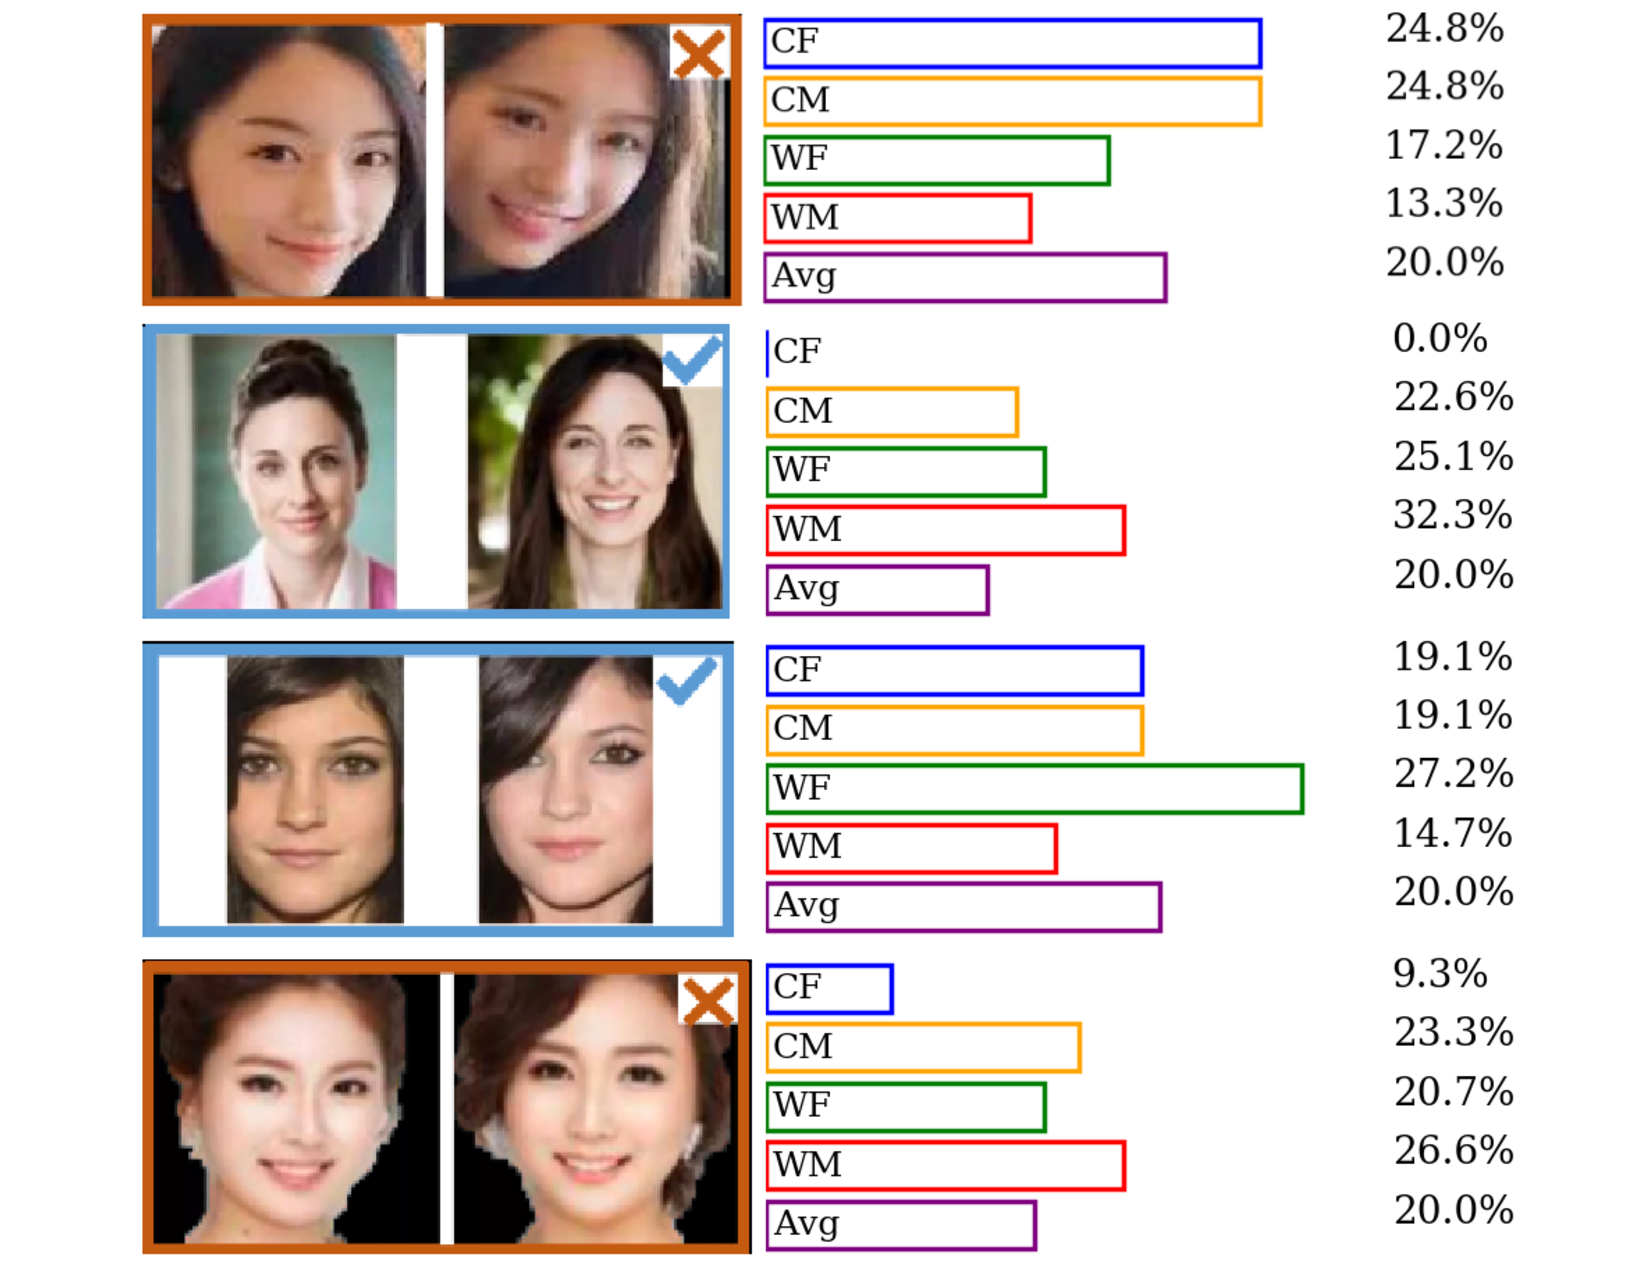
\includegraphics[width=\linewidth] {images/human_eval.pdf}
		\caption{\small{\textbf{Qualitative results of human assessment.} $\checkmark$ for \emph{match}; $\times$ for \emph{non-match}, which scores plotted next to each. Humans tend to be more successful at recognizing their own subgroup, with few exceptions (bottom). }}
		% (\eg bottom row). } Result summary in Table~\ref{tab:human-eval}.
		\label{fig:human-eval} 
		\vspace{-5mm}
\end{figure} 

% \vspace{-5pt}
\subsection{Human evaluation}
 Quantitative and qualitative results are in Table~\ref{tab:humsn-eval-results} and Fig.~\ref{fig:human-eval}, respectfully. One might expect that the most exposure to others would be within the same subgroup, and, therefore, would be best at labeling their own. Secondarily, they would be best at labeling images of the same ethnicity, but opposite gender. Our findings concur. Each subgroup is best at labeling their type, and then second best at labeling the same ethnicity but opposite sex. Interestingly, each group of images is best tagged by the corresponding subgroup, with the second-to-best having the same ethnicity and opposite gender. On average, subgroups are comparable at labeling images. 



